\section{To go further : configuration signal exchanges between FPGA and GNU Radio}

\subsection{SystemVerilog parameters}
When instantiating the IP in the subsystem, you are allowed to define the values of a few \textit{SystemVerilog parameters} for the top-level module of the preamble detector, as shown in Figure \ref{fig:pd_hard_param}. Those parameters described in the Table \ref{table:pd_hard_param}.

\begin{figure}[!h]
    \centering
    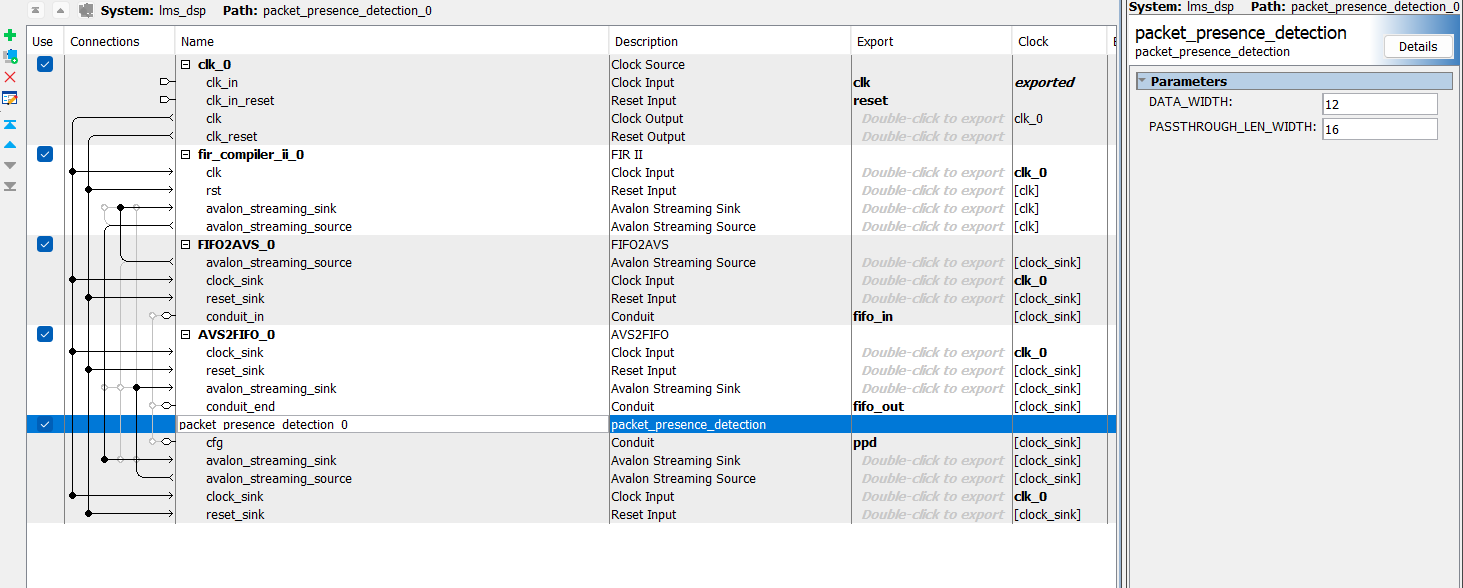
\includegraphics[width=\linewidth]{figures/ppd_detect_qsys_config.PNG}
    \caption{SystemVerilog parameters of the packet presence detector in QSYS.}
    \label{fig:pd_hard_param}
\end{figure}

\begin{table}[!h]
\centering
\begin{tabular}{|p{0.36\linewidth}|p{0.48\linewidth}|p{0.08\linewidth}|}
\hline
Parameter & Description & Default value \\
\hline
\textsc{DATA\_WIDTH} & Bit width of the samples & 12 \\
\hline
\textsc{PASSTHROUGH\_LEN\_WIDTH} & Bit width of the configurable number of samples to pass-through once the threshold is reached & 16 \\
\hline
\end{tabular}
\caption{SystemVerilog parameters of the \texttt{preamble\_detector} IP}
\label{table:pd_hard_param}
\end{table}

\subsection{Configuration signals}
\begin{sloppypar}
Additionally, there are several configuration signals that can be changed during operation from GNU Radio for better flexibility. Those configuration signals are listed in Table \ref{table:pd_soft_param}, you can trace them in the VHDL code, they are coming from the \texttt{fpgacfg} module defined in \texttt{LimeSDR-Mini\_lms7\_lelec210x/src/spi/fpgacfg.vhd} and located in the design hierarchy at \texttt{lms7\_trx\_top/inst0\_nios\_cpu/cfg\_top\_inst1/fpgacfg\_inst0}, as shown in Figure \ref{fig:design_hier_fpgacfg}.
\end{sloppypar}

This module contains a RAM with 16-bit words that retains the configuration of various elements of the FPGA. We used available addresses to put our custom configuration, the address map is written in the repo README. There are default values assigned at reset for the memory bits (Figure \ref{fig:design_hier_fpgacfg}) but they can be changed with a write operation.

\begin{table}[!h]
\centering
\begin{tabular}{|p{0.22\linewidth}|p{0.25\linewidth}|p{0.34\linewidth}|p{0.08\linewidth}|}
\hline
Configuration signal & Description & Allowed values\\
\hline
\texttt{cfg\_enable} & Enable or disable the PPD. & $\left\{0,1\right\}$ \\
\hline
\texttt{cfg\_clear\_} & Clear the delay lines of the dual running sum. & $\left\{0,1\right\}$ \\
\hline
\texttt{cfg\_PASSTHROUGH\_LEN} & Number of samples to pass-through after a start flag has been added. Avoid any retriggering of this flag meanwhile. & $\left[1,2^{\textsc{PASSTHROUGH\_LEN\_WIDTH}}-1\right]$ \\
\hline
\texttt{cfg\_THRESHOLD} & Value to multiply the normalized result of the long-term sum, before comparison. & $\left[1,2^{8}-1\right]$ \\
\hline
\end{tabular}
\caption{Configuration signals \texttt{packet\_presence\_detection} IP}
\label{table:pd_soft_param}
\end{table}

\begin{figure}[!h]
    \centering
    \includegraphics[width=0.3\linewidth]{figures/design_hierarchy_fpgacfg.PNG}
    \includegraphics[width=0.6\linewidth]{figures/design_hierarchy_fpgacfg_both.PNG}
    \caption{Configuration signal location in the design hierarchy (left). Assignment and reset values for the DSP configuration signals (right).}
    \label{fig:design_hier_fpgacfg}
\end{figure}

\subsubsection{Read/write operations of the configuration signals from GNU Radio}
The GNU Radio block of the LimeSDR-Mini uses a C++ library called \textit{LimeSuite} in order to write data to the FPGA configuration memory. In the following paragraph, the configuration flow inside LimeSuite and the hardware is briefly described.

\begin{sloppypar}
\paragraph{gr-limesdr GUI interface}
In our custom version of the limeSDR GNU Radio block, we added fields to configure the hardware preamble detector. To do so, we modified the file \texttt{gr-limesdr/grc/limesdr\_fpga\_source.block.yml} and added a GUI callback function named \texttt{set\_dspcfg\_preamble}. This function is in turn defined in \texttt{gr-limesdr/lib/source\_impl.cc} and \texttt{gr-limesdr/lib/device\_handler.cc}. Please take a look at the end of \texttt{device\_handler.cc} and understand the functions we added. At the core of all of them, we use \texttt{modify\_spi\_reg\_bits}, shown in Figure \ref{fig:modify_spi_reg_bits}, that uses LimeSuite \texttt{LMS\_WriteFPGAReg} function. Pay attention to the arguments and try to make the link with the configuration memory of the FPGA, the input structures are defined in \texttt{gr-limesdr/lib/fpga\_register\_map.h}.
\end{sloppypar}

\begin{figure}[!h]
    \centering
    \includegraphics[width=\linewidth]{figures/grlimesdr_write_fpgacfg.PNG}
    \caption{Software interface between GNU Radio and LimeSuite.}
    \label{fig:modify_spi_reg_bits}
\end{figure}

\paragraph{NIOS Interface}
When calling \texttt{LMS\_WriteFPGAReg}, the functions wrap the address and value of the register we wish to configure inside a packet that is transmitted through USB. The complete callstack inside the library is described in the repo README. The USB interface is connected to an FTDI Chip which is in turn interfaced with the FPGA, as shown in Figure \ref{fig:limesdr_mini_schematic}.

Inside the FPGA, we have:
\begin{enumerate}
    \item An FTDI arbitrer that decodes a first part of the packet header to forward it through a configuration FIFO (\texttt{EP02\_fifo}) towards the NIOS subsystem. This arbitration is necessary as we have two other FIFOs coming from the NIOS subsystem and the RX data path (\texttt{EP83\_fifo} and \texttt{EP82\_fifo} respectively).
    \item A NIOS Softcore processor instantiated inside the FPGA reads the FIFO and decodes the second part of the packet header, it then forwards the packet data to through an SPI Master.
    \item An SPI Slave is connected with the configuration memory and writes the received data at the correct address.
\end{enumerate}

\begin{bclogo}[couleur = gray!20, arrondi = 0.2, logo=\bcinfo]{Additional resources}
To help you understand this complex path, we provided you with resources you can find on moodle or \texttt{LimeSDR-Mini\_lms7\_lelec210x/doc/} folder. The file \texttt{FPGA\_config\_path.pdf} with annotations referring to the above paragraph should be helpful, several elements have been hidden to ease the reading. You can also use freely the RTL viewer to skim through the design hierarchy graphically instead of opening files, see Figure \ref{fig:rtl_viewer} for further details.
\end{bclogo}

\begin{figure}[!h]
    \centering
    \includegraphics[width=0.7\linewidth]{figures/limesdrmini_schematic.png}
    \caption{Location of the different chips on the LimeSDR-Mini board.}
    \label{fig:limesdr_mini_schematic}
\end{figure}

\begin{figure}[!h]
    \centering
    \includegraphics[width=0.7\linewidth]{figures/rtl_viewer.png}
    \caption{In order to use the RTL viewer, first elaborate the design (1) then right click on the design element you want view (2).}
    \label{fig:rtl_viewer}
\end{figure}
